
\documentclass[10pt,a4paper]{article}
\usepackage[T1]{fontenc}
\usepackage{tikz}
\usepackage[margin=1cm]{geometry}
\begin{document}
\section*{Step-by-Step Deletion Process in a Binary Search Tree (BST)}
This document presents the step-by-step process of deleting nodes from a Binary Search Tree (BST). Each step includes a visualization of the tree before and after the deletion of a specific node. Nodes are removed according to BST deletion rules, ensuring that the tree's properties are maintained.

\subsection*{Process Overview}
For each deletion operation:
\begin{itemize}
    \item The tree before deletion is shown, with the node to be deleted highlighted in \textcolor{red}{red}.
    \item The tree after deletion is displayed, illustrating the new structure of the BST.
\end{itemize}


\begin{figure}[h!]
\centering

\begin{minipage}{0.8\textwidth}
    \centering
    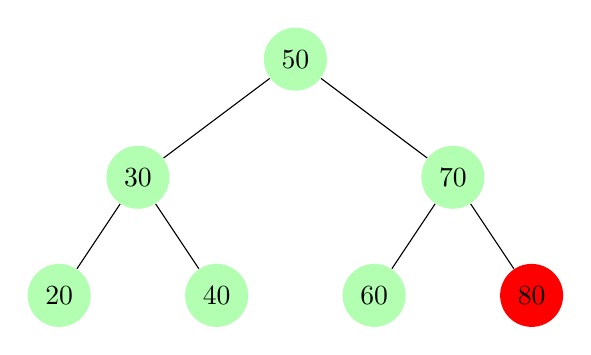
\begin{tikzpicture}[level distance=15mm, sibling distance=20mm]
        \tikzstyle{every node}=[circle,inner sep=1pt, minimum size=8mm]
        \tikzstyle{level 1}=[sibling distance=40mm, set style={{every node}+=[fill=green!30]}]
        \tikzstyle{level 2}=[sibling distance=20mm, set style={{every node}+=[fill=green!30]}]
        \tikzstyle{level 3}=[sibling distance=15mm, set style={{every node}+=[fill=green!30]}]
        \tikzstyle{level 4}=[sibling distance=10mm, set style={{every node}+=[fill=green!30]}]
        \node [fill=green!30] {50} child {node [fill=green!30] {30} child {node [fill=green!30] {20} } child {node [fill=green!30] {40} }} child {node [fill=green!30] {70} child {node [fill=green!30] {60} } child {node [fill=red] {80} }};
    \end{tikzpicture}
    \caption{Tree before deletion (Node to delete in red)}
\end{minipage}
\vspace{5cm}

\begin{minipage}{0.8\textwidth}
    \centering
    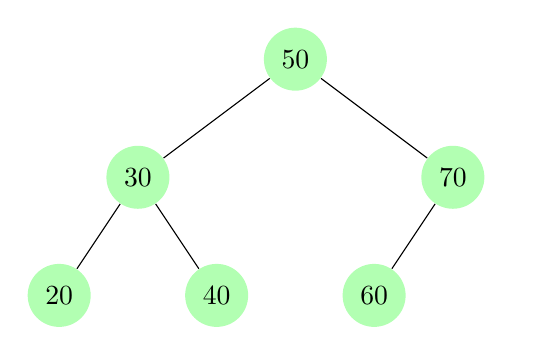
\begin{tikzpicture}[level distance=15mm, sibling distance=20mm]
        \tikzstyle{every node}=[circle,inner sep=1pt, minimum size=8mm]
        \tikzstyle{level 1}=[sibling distance=40mm, set style={{every node}+=[fill=green!30]}]
        \tikzstyle{level 2}=[sibling distance=20mm, set style={{every node}+=[fill=green!30]}]
        \tikzstyle{level 3}=[sibling distance=15mm, set style={{every node}+=[fill=green!30]}]
        \tikzstyle{level 4}=[sibling distance=10mm, set style={{every node}+=[fill=green!30]}]
        \node [fill=green!30] {50} child {node [fill=green!30] {30} child {node [fill=green!30] {20} } child {node [fill=green!30] {40} }} child {node [fill=green!30] {70} child {node [fill=green!30] {60} } child[fill=none] {edge from parent[draw=none]}};
    \end{tikzpicture}
    \caption{Tree after deletion}
\end{minipage}
\vspace{1cm}

\end{figure}
\newpage

\begin{figure}[h!]
\centering

\begin{minipage}{0.8\textwidth}
    \centering
    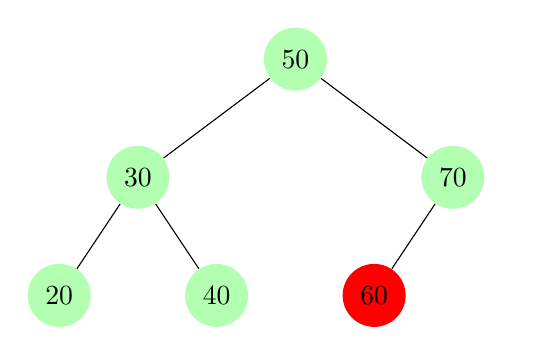
\begin{tikzpicture}[level distance=15mm, sibling distance=20mm]
        \tikzstyle{every node}=[circle,inner sep=1pt, minimum size=8mm]
        \tikzstyle{level 1}=[sibling distance=40mm, set style={{every node}+=[fill=green!30]}]
        \tikzstyle{level 2}=[sibling distance=20mm, set style={{every node}+=[fill=green!30]}]
        \tikzstyle{level 3}=[sibling distance=15mm, set style={{every node}+=[fill=green!30]}]
        \tikzstyle{level 4}=[sibling distance=10mm, set style={{every node}+=[fill=green!30]}]
        \node [fill=green!30] {50} child {node [fill=green!30] {30} child {node [fill=green!30] {20} } child {node [fill=green!30] {40} }} child {node [fill=green!30] {70} child {node [fill=red] {60} } child[fill=none] {edge from parent[draw=none]}};
    \end{tikzpicture}
    \caption{Tree before deletion (Node to delete in red)}
\end{minipage}
\vspace{5cm}

\begin{minipage}{0.8\textwidth}
    \centering
    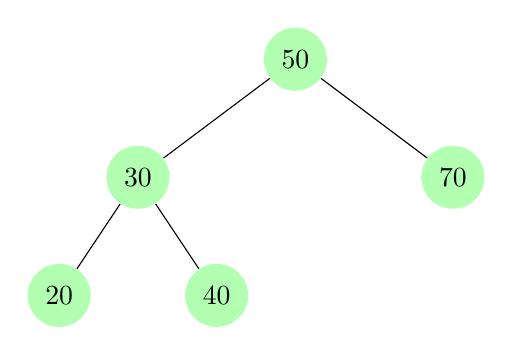
\begin{tikzpicture}[level distance=15mm, sibling distance=20mm]
        \tikzstyle{every node}=[circle,inner sep=1pt, minimum size=8mm]
        \tikzstyle{level 1}=[sibling distance=40mm, set style={{every node}+=[fill=green!30]}]
        \tikzstyle{level 2}=[sibling distance=20mm, set style={{every node}+=[fill=green!30]}]
        \tikzstyle{level 3}=[sibling distance=15mm, set style={{every node}+=[fill=green!30]}]
        \tikzstyle{level 4}=[sibling distance=10mm, set style={{every node}+=[fill=green!30]}]
        \node [fill=green!30] {50} child {node [fill=green!30] {30} child {node [fill=green!30] {20} } child {node [fill=green!30] {40} }} child {node [fill=green!30] {70} };
    \end{tikzpicture}
    \caption{Tree after deletion}
\end{minipage}
\vspace{1cm}

\end{figure}
\newpage

\end{document}
